\documentclass{elsarticle}
\biboptions{numbers,sort&compress}
\usepackage[utf8]{inputenc}
\usepackage{amsmath} % mates
\usepackage{graphicx} % poner figuras
\usepackage[spanish,es-tabla]{babel} % nombre tablas
\usepackage{caption}
\usepackage{subcaption}
\usepackage{natbib}
\usepackage{listings} % listings
\usepackage{color} %colores
\lstset{
    language=bash,
    inputencoding=utf8,
    literate={á}{{\'a}}1 {ã}{{\~a}}1 {é}{{\'e}}1 {ú}{{\'u}}1 {ó}{{\'o}}1 {í}{{\'i}}1 {ñ}{{\~n}}1,
}


\definecolor{mypink}{rgb}{0.976, 0.462, 0.847}
\definecolor{mygray}{rgb}{0.976, 0.980, 0.980}
\definecolor{myblue}{rgb}{0.258, 0.682, 1}
\definecolor{mypink2}{rgb}{0.525, 0.054, 0.4}
\lstset{ 
  backgroundcolor=\color{mygray},
  commentstyle=\color{myblue},
  keywordstyle=\color{mypink}, 
  numberstyle=\tiny\color{mypink}
  stringstyle=\color{mypink2}, 
  breaklines=true,
}

\title{Proyecto Final: Conductancia en cátodos de carbono con nanopartículas de platino depositadas \tnoteref{t1}}
\tnotetext[t1]{Proyecto Final: Simulación Computacional de Nanomateriales}
\author{Eduardo Navarro}


\ead{eduardo.navarror@uanl.edu.mx}


\date{Otoño 2021}

\address[1]{Maestría en Ciencias de la Ingeniería con Orientación en Nanotecnología, \\ Facultad de Ingenieería Mecánica y Eléctrica, \\ Universidad Autónoma de Nuevo León}

\begin{document}

\begin{abstract}
En el presente trabajo se pretende explicar la conductancia en función de la resistividad de los nanomateriales de carbono dopados con nanopartículas como cátodos. Además de que se describen algunas de las propiedades por las cuales se debe este comportamiento para posteriormente lograr una simulación apropiada de este fenómeno.  
\end{abstract}

\begin{keyword}
Nanopartículas, platino, cátodo, carbono, Conductancia. 
\end{keyword}

\maketitle


\section{Introducción}

La nanotecnología nos ayuda a mejorar las propiedades de los materiales. Desde hace algunos años los nanomateriales han servido como los nuevos bloques de construcción para el aprovechamiento de las energías. Por ejemplo investigaciones recientes nos han mostrado que una película de nanotubos de carbono puede remplazar dos de las capas que se usan normalmente en las celdas solares junto con un aumento en el rendimiento y una reducción del costo. Los materiales de carbono como el grafito presentan una ventaja por su alta área superficial lo que incrementa su actividad catalítica. Esto a su vez permite experimentar con otras formas del carbono como lo son las nanoestructuras de grafito, carbón, fullerenos, nanotubos de carbono y grafeno \cite{calandraimg}.  El material catódico (figura \ref{fig1}) generalmente es requerido para proveer una alta corriente de intercambio. Esto significa que la superficie catalítica disponible juega un papel importante a la hora de determinar la corriente general del dispositivo. Es por ello que la preparación de los electrodos con alta área superficial es deseable ya que esto asegura un mayor número de densidad en los sitios catalíticos activos \cite{calandraimg}. Las nanopartículas metálicas depositadas sobre el cátodo tienen una influencia final en las propiedades y estructura del cátodo dando como resultado en última instancia, el rendimiento final del dispositivo.

Los nanotubos de carbono tienen excelentes propiedades eléctricas incluyendo el transporte de cargas y conservación de spin en adición a altas capacidades de corriente de carga y alta reactividad química. La mayoría de las aplicaciones, tales como dispositivos de detección, fotovoltaicos y emisores de campo, requieren conjuntos macro o mesoscópicos de nanotubos de carbono donde las propiedades funcionales de los nanotubos individuales se conservan y se traducen en las propiedades macroscópicas del dispositivo. Idealmente, el proceso de ensamblaje debería conducir a la formación de redes homogéneas de nanotubos de carbono con estructuras bien definidas que podrían sintonizarse y controlarse utilizando diferentes condiciones de ensamblaje \cite{Marshgrap}.

\begin{figure}[ht!]
	\centering
		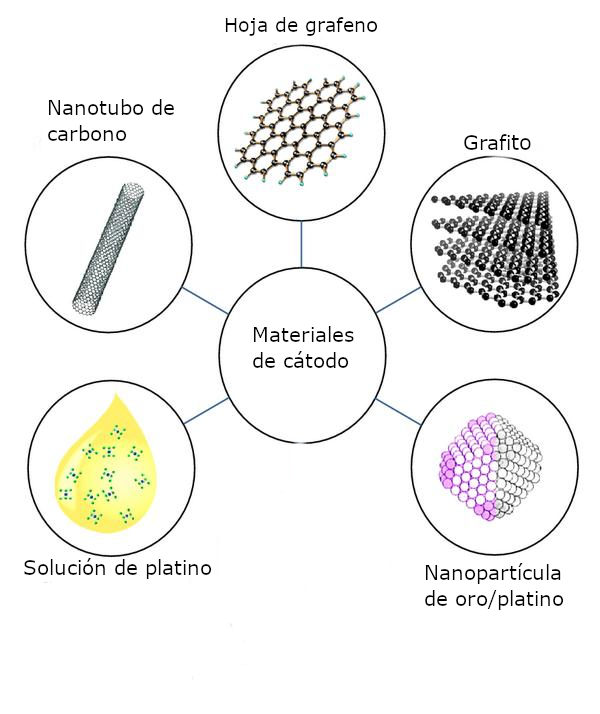
\includegraphics[scale=1]{catodos.png}
	\caption{Ejemplo de materiales de carbono usados como cátodos y algunas nanopartículas metálicas. Basado en \citet{calandraimg}(2010)}
	\label{fig1}
\end{figure}

\section{Antecedentes}

Las propiedades eléctricas de la red ensamblada vistas mediante la caracterización estructural macroscópica y microscópica sirven como intento de correlacionar las propiedades eléctricas con su morfología física. Mediante el uso de nanotubos de carbono funcionalizados se han introducido interacciones específicas entre las nano partículas y el nanotubo donde se ha investigado el impacto que esto tiene en la percolación de electrones a través del sistema. En el estudio que se realizó fue importante obtener un sistema disperso de nanotubos, donde el nanotubo se dejó inalterado mediante la adición de surfactantes. La presencia de este surfactante en el sistema afecta significativamente la estructura formada en la interface. Como los nanotubos de carbono tienen una baja solubilidad se utiliza un método para las suspensiones a ciertas concentraciones. Este método de funcionalización además permite la solubilización de los nanotubos en ausencia del surfactante. Estos tratamientos llevan a incrementos en solubilidad y estabilidad de la suspensión. Los grupos carboxílicos (–COOH) y los grupos tiol (–SH) son capaces de unirse a átomos de oro y por lo tanto; pueden utilizarse para anclar nanopartículas. Estos nanotubos de carbono independientemente de su función forman películas consistentemente \cite{Marshgrap}. 

Para el análisis de la cobertura del área del nanotubo por las nanopartículas se utilizan imágenes de un microscopio electrónico de transmisión (TEM). Por lo general el espesor de los nanotubos de carbono es solo de unas decenas de nanómetros y puede pensarse como una monocapa mezclada de dos componentes. Las islas de nanopartículas son 2D en la naturaleza y raramente exhiben apilamiento vertical. Esto es consistente con su ensamblaje completamente restringido dentro de la interfaz líquido-líquido. Los nanotubos de carbono están entretejidos, pero siguen siendo esencialmente en cuanto a estructura, 2D. Por lo que se considera morfológicamente una estructura cuasi-2D. El número de nanopartículas depositadas sobre la película se mide como una fracción del umbral de la superficie cubierta analizando los datos del TEM, esta varía de escasa a densa, manteniendo la morfología 2D. Después de un cierto umbral de concentración, las nanopartículas se segregan de los nanotubos formando islas muy compactas. La dispersión en los datos es indicativa del rango de coberturas de partículas obtenidas. Es interesante que a pesar de las observaciones en el incremento del contenido de nanopartículas en el filme la red subyacente de nanotubos de carbono permanece cualitativamente sin cambios en términos de densidad de nanotubos por unidad de área independientemente de la concentración de los nanotubos \cite{Marshgrap}.


\begin{figure}[ht!]
	\centering
		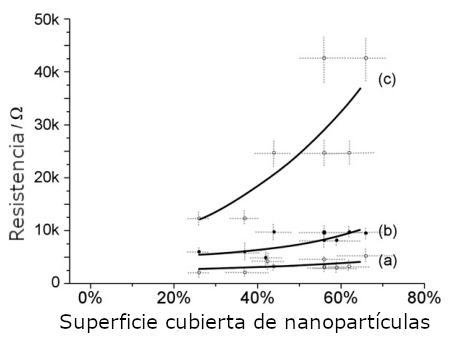
\includegraphics[scale=2]{graficaarea.png}
	\caption{Resistencia del nanomaterial contra el área cubierta por la nanopartícula. (a) separación de electrodos de 5 micrones, (b) separación de 10 micrones, y (c) 20 micrones. Basado en \citet{Marshgrap} (2008)}
	\label{fig2}
\end{figure}


Para medir la conductancia se muestran los datos de resistencia en función del contenido de nanopartículas (figura \ref{fig2}). Se muestra la resistencia (en lugar de la resistividad) específicamente para resaltar el efecto de escala. Los datos se muestran para espacios estrechos de electrodos con separaciones de 5, 10 y 20 micrones. Se notó que una pequeña cantidad de nanopartículas conduce a una disminución de la resistencia. Sin embargo, a medida que aumenta la fracción de nanopartículas en la película, la resistencia aumenta nuevamente. Este efecto se vuelve más pronunciado en espacios más grandes. Se cree que esto está relacionado con la compleja mezcla de morfologías de unión presentes en las redes. La filtración de los portadores de carga a través de la red puede describirse mediante una estructura de ramificación de vías de interconexión e interpenetración. La contribución resistiva de los nanotubos se puede descartar ya que es probable que sea en gran medida de naturaleza balística y por lo tanto, se puede suponer que no es resistiva \cite{Marshgrap}.

\begin{table}[h!]
\centering
\caption{Conductividad eléctrica de catalizadores de monoplatino. Basado en \citet{Bogdanovskayatab} (2021)}
\label{tabla1}
\begin{tabular}{|c|r|r|r|}
\hline
\textbf{Catalizador} & \textbf{\begin{tabular}[c]{@{}c@{}}Resistencia \\ específica\\  R, $\Omega$ cm\end{tabular}} & \textbf{\begin{tabular}[c]{@{}c@{}}Densidad,\\  g/cm3\end{tabular}} & \textbf{\begin{tabular}[c]{@{}c@{}}Conductancia \\ específica\\  k, S/cm\end{tabular}} \\ \hline
Pt/CNTinitial & 5.90 & 1.69 & 0.17 \\ \hline
Pt/CNTHNO3 & 4.50 & 1.12 & 0.22 \\ \hline
Pt/CNTHNO3+N & 6.28 & 1.96 & 0.16 \\ \hline
Pt/CNTHNO3+P & 4.70 & 1.00 & 0.21 \\ \hline
Pt/CNTHNO3+NP & 5.50 & 1.61 & 0.18 \\ \hline
\end{tabular}
\end{table}

Como hemos podido observar la conductividad eléctrica es una de las características más importantes. Por ejemplo, para el platino se tiene la conductividad eléctrica de los catalizadores que se calcularon en base a la resistencia medida como se muestra en la tabla \ref{tabla1}. Esta propiedad nos indica que el platino cuenta con una buena conductancia y es por ello que es de gran interés para el estudio en general \cite{Bogdanovskayatab}.

\section{Propuesta}
Se planea simular los resultados vistos en la figura \ref{fig2} donde se tiene la resistencia en función de la superficie cubierta, para tratar de lograr resultados similares y adecuados. Primero se evaluó el fenómeno observando las variables más importantes las cuales son; la distancia que separan a los cátodos y la superficie cubierta con las nanopartículas dentro de las cuales se aprecia como aumenta la resistencia a medida que ambas propiedades aumentan llegando a tomar valores similares dentro de regiones con mayor cobertura. En base a lo anterior se propuso la fórmula \ref{funcion} donde la molécula es el número atómico, la superficie es el porcentaje de superficie cubierta por la nanopartícula, la c es una constante arbitraria y la separación es la distancia que separa al electrodo.

\begin{equation}
Resistencia=(mol\acute{e}cula*superficie)^c/(1/separaci\acute{o}n)
\label{funcion}
\end{equation}

Primero en el código se añadieron los parámetros a tomar en cuenta como la superficie cubierta y la separación, después se añadieron unos \texttt{for} para tomar cada valor, aplicar la fórmula \ref{funcion}, separarlos con un \texttt{if} para cada nivel de separación y añadirlo todo a un \texttt{data.frame} base.

\begin{lstlisting} [language=R, caption= Código para la obtención de los valores de resistencia para diversos porcentajes.] 
molecula<-c(78)#Número atómico
superficie_cubierta<-c(20,30,40,50,60,70) #Norma de área
separacion<-c(5,10,15)#Norma de separación

j<-1:2 #Repeticiones

datos<-data.frame()

for (rep in j) {

for (mole in molecula) {
  
  for (superficie in superficie_cubierta) {
    
    for (sepa in separacion) {
      
      if (sepa<=5){ #Genera para distancia de 5
        resistividad<-((mole*superficie)*0.2)/(1/sepa)}
      
      else if(sepa<=10){ #Genera para distancia de 10
        resistividad<-((mole*superficie)*0.2)/(1/sepa)}
      
      else if(sepa<=15){ #Genera para distancia de 15
         resistividad<-((mole*superficie)*0.52)/(1/sepa)}
      
      resultado<-c(mole,superficie,sepa,resistividad)# Añadir al data.frame
      datos=rbind(datos,resultado)
    }
  }
}
}
\end{lstlisting}

Después se creó un generador de área en base a una matriz \cite{jvanwijk_oliver_2019}. Donde se genera de acuerdo a una probabilidad dada a dimensiones dadas añadiendo todo a otro \texttt{data.frame} para posteriormente combinar ambos y obtener unos resultados semejantes a la figura \ref{fig2}.

\begin{lstlisting} [language=R, caption= Código para la obtención de matrices de área.] 

area<-data.frame()

nsim <- 10 #Cuantos rbinom existen
n <- 10 #Largo de lado de matriz
size = 1 #Solo 0 y 1
secuen = c(0.2,0.2,0.2,0.3,0.3,0.3,0.4,0.4,0.4,0.5,
0.5,0.5,0.6,0.6,0.6,0.7,0.7,0.7) # Probabilidades de llenado de matriz

for (repe in j) {
  
for (prob in secuen) {
  
  matriz <- matrix(ncol = nsim, nrow = n)#Genera matriz
  for(i in seq(nsim)) #Itera de 1 a nsim
    matriz[, i] <- rbinom(n, size = size, prob = prob)
  suma<-sum(matriz)#"Superficie cubierta"
  
  resul<-c(suma)
  area=rbind(area,resul)#Guardar resultados en data.frame
  
  print(suma)
  
}
}
df<-cbind(datos, area) #Combinar los data.frames

names(df) = c("molecula", "superficie", "separacion", "resistencia","recubierta")
\end{lstlisting}

Se combinaron ambos \texttt{data.frame} para obtener una relación entre la norma y el área generada por la matriz.

\section{Resultados}

Se obtuvo la siguiente gráfica como resultado, que es muy semejante a la observada en la figura \ref{fig2}.


\begin{figure} [h!]% figura
\renewcommand{\figurename}{Gráfica}
    \centering
    \caption{ Resistencia del nanomaterial contra el área cubierta por la nanopartícula.}
    \label{grafica1}
    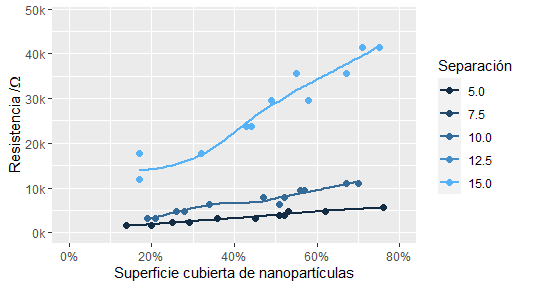
\includegraphics[width=85mm]{grafica1.png} % archivo
\end{figure}

\begin{lstlisting} [language=R, caption= Código para la obtención de la gráfica.] 
ggplot(df, aes(x= recubierta, y= resistencia, color=separacion)) + 
  geom_point(size=2)+
  geom_smooth(aes(group = separacion),method = "loess", se=FALSE, formula =y ~ x)+#Línea de tendencia
  guides(scale = "10", color=guide_legend(title = "Separación"))+
  theme(plot.title = element_text(hjust = 0.5))+
  scale_x_continuous(label = unit_format(unit = "%", scale = 1, sep = ""),limits=c(0, 80)) + # % en las etiquetas 
  scale_y_continuous(label = unit_format(unit = "k", scale = 1e-3, sep = ""),limits = c(0,48000))+# k en las etiquetas
  labs(x="Superficie cubierta de nanopartículas")+
  ylab(expression("Resistencia"~"/"*Omega*"")) #Símbolo Omega

\end{lstlisting}

\begin{table}[h!]
\centering
\caption{Ejemplo de datos obtenidos}
\label{tabla2}
\begin{tabular}{|r|r|r|r|r|}
\hline
\multicolumn{1}{|c|}{\textbf{Molécula}} & \multicolumn{1}{c|}{\textbf{Superficie}} & \multicolumn{1}{c|}{\textbf{Separación}} & \multicolumn{1}{c|}{\textbf{Resistencia}} & \multicolumn{1}{c|}{\textbf{Recubierta}} \\ \hline
78 & 20 & 5 & 1560 & 18 \\ \hline
78 & 20 & 10 & 3120 & 18 \\ \hline
78 & 20 & 15 & 12168 & 22 \\ \hline
78 & 30 & 5 & 2340 & 29 \\ \hline
78 & 30 & 10 & 4680 & 28 \\ \hline
78 & 30 & 15 & 18252 & 32 \\ \hline
\end{tabular}
\end{table}

\begin{lstlisting} [language=R, caption= Ejemplo de matriz obtenida.] 
      [,1] [,2] [,3] [,4] [,5] [,6] [,7] [,8] [,9] [,10]
 [1,]    1    1    1    0    1    0    1    1    1     1
 [2,]    0    1    1    1    1    1    0    0    0     0
 [3,]    0    0    1    0    1    1    0    0    1     1
 [4,]    0    1    1    1    1    1    1    0    0     1
 [5,]    1    1    0    0    1    1    1    1    1     0
 [6,]    0    1    1    1    0    1    1    1    1     1
 [7,]    1    1    1    0    1    0    1    1    1     0
 [8,]    1    1    1    1    0    1    1    1    1     0
 [9,]    1    1    1    0    1    1    1    1    1     0
[10,]    1    1    0    1    1    1    1    1    1     1
\end{lstlisting}

Se procedió a realizarlo con más repeticiones para obtener datos estadísticos relevantes.
\newpage
\begin{figure} [h!]% figura
\renewcommand{\figurename}{Gráfica}
    \centering
    \caption{ Resistencia del nanomaterial contra el área cubierta por la nanopartícula para 5 de separación.}
    \label{grafica2}
    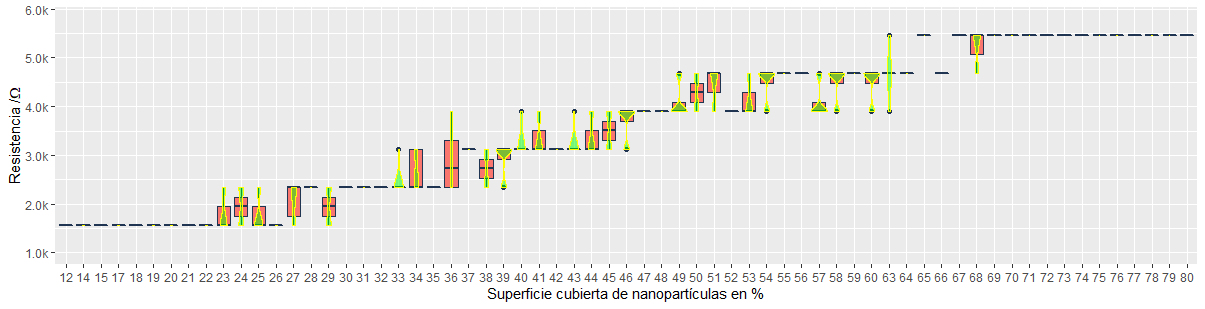
\includegraphics[width=120mm]{grafica2.png} % archivo
\end{figure}

\begin{figure} [h!]% figura
\renewcommand{\figurename}{Gráfica}
    \centering
    \caption{ Resistencia del nanomaterial contra el área cubierta por la nanopartícula para 10 de separación.}
    \label{grafica3}
    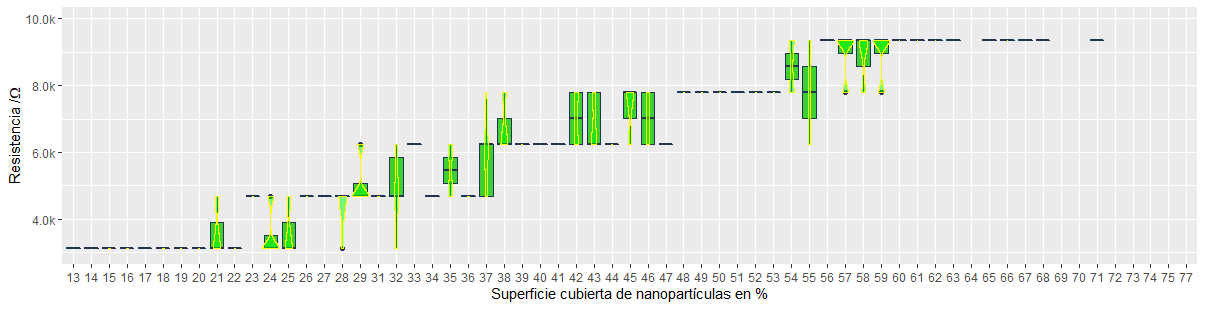
\includegraphics[width=120mm]{grafica3.png} % archivo
\end{figure}

\begin{figure} [h!]% figura
\renewcommand{\figurename}{Gráfica}
    \centering
    \caption{ Resistencia del nanomaterial contra el área cubierta por la nanopartícula para 15 de separación.}
    \label{grafica4}
    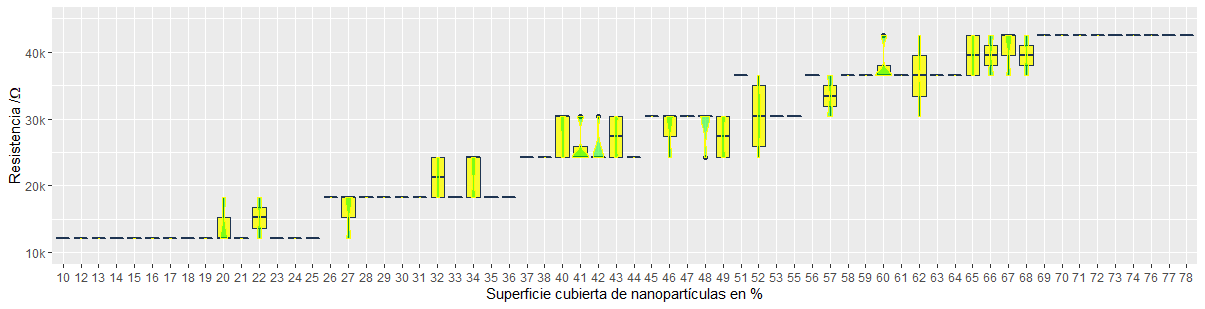
\includegraphics[width=120mm]{grafica4.png} % archivo
\end{figure}

\begin{table}[h!]
\centering
\caption{Ejemplo de datos estadísticos para 5 de separación}
\label{tabla3}
\begin{tabular}{|l|l|l|l|l|l|}
\hline
\multicolumn{1}{|c|}{Superficie} & \multicolumn{1}{c|}{Promedio} & \multicolumn{1}{c|}{\begin{tabular}[c]{@{}c@{}}Desviación\\ estándar\end{tabular}} & \multicolumn{1}{c|}{Varianza} & \multicolumn{1}{c|}{Mediana} & \multicolumn{1}{c|}{\begin{tabular}[c]{@{}c@{}}Rango\\ intercuartil\end{tabular}} \\ \hline
23 & 1820.0 & 450.3 & 202800.0 & 1560.0 & 390.0 \\ \hline
24 & 1950.0 & 551.5 & 304200.0 & 1950.0 & 390.0 \\ \hline
25 & 1782.8 & 380.6 & 144857.1 & 1560.0 & 390.0 \\ \hline
27 & 2080.0 & 402.8 & 162240.0 & 2340.0 & 585.0 \\ \hline
29 & 1950.0 & 551.5 & 304200.0 & 1950.0 & 390.0 \\ \hline
\end{tabular}
\end{table}

\newpage

\begin{table}[h!]
\centering
\caption{Ejemplo de datos estadísticos para 10 de separación}
\label{tabla4}
\begin{tabular}{|l|l|l|l|l|l|}
\hline
\multicolumn{1}{|c|}{Superficie} & \multicolumn{1}{c|}{Promedio} & \multicolumn{1}{c|}{\begin{tabular}[c]{@{}c@{}}Desviación\\ estándar\end{tabular}} & \multicolumn{1}{c|}{Varianza} & \multicolumn{1}{c|}{Mediana} & \multicolumn{1}{c|}{\begin{tabular}[c]{@{}c@{}}Rango\\ intercuartil\end{tabular}} \\ \hline
21 & 3640.0 & 900.6 & 811200.0 & 3120.0 & 780.0 \\ \hline
24 & 3510.0 & 780.0 & 608400.0 & 3120.0 & 390.0 \\ \hline
25 & 3640.0 & 900.6 & 811200.0 & 3120.0 & 780.0 \\ \hline
29 & 5070.0 & 780.0 & 608400.0 & 4680.0 & 390.0 \\ \hline
32 & 4940.0 & 1174.3 & 1379040.0 & 4680.0 & 1170.0 \\ \hline
\end{tabular}
\end{table}

\begin{table}[h!]
\centering
\caption{Ejemplo de datos estadísticos para 15 de separación}
\label{tabla5}
\begin{tabular}{|l|l|l|l|l|l|}
\hline
\multicolumn{1}{|c|}{Superficie} & \multicolumn{1}{c|}{Promedio} & \multicolumn{1}{c|}{\begin{tabular}[c]{@{}c@{}}Desviación\\ estándar\end{tabular}} & \multicolumn{1}{c|}{Varianza} & \multicolumn{1}{c|}{Mediana} & \multicolumn{1}{c|}{\begin{tabular}[c]{@{}c@{}}Rango\\ intercuartil\end{tabular}} \\ \hline
20 & 14196.0 & 3512.5 & 12338352.0 & 12168.0 & 3042.0 \\ \hline
22 & 15210.0 & 4302.0 & 18507528.0 & 15210.0 & 3042.0 \\ \hline
27 & 16224.0 & 3512.5 & 12338352.0 & 18252.0 & 3042.0 \\ \hline
32 & 21294.0 & 3512.5 & 12338352.0 & 21294.0 & 6084.0 \\ \hline
34 & 21902.4 & 3332.3 & 11104517.0 & 24336.0 & 6084.0 \\ \hline
\end{tabular}
\end{table}

Para la norma se realizó la prueba de normalidad de Shapiro–Wilk\cite{shapiro}, la prueba estadística de Kruskal-Wallis \cite{Kruskall} y la prueba de grupos de Wilcox \cite{pairwise}.

\begin{table}[h!]
\centering
\caption{Resultados de la prueba Shapiro–Wilk.}
\label{tabla6}
\begin{tabular}{|c|r|r|}
\hline
Separación & \multicolumn{1}{c|}{W} & \multicolumn{1}{c|}{P} \\ \hline
5 & 0.9059 & $2.67\times 10^{-9}$ \\ \hline
10 & 0.9059 & $2.67\times 10^{-9}$ \\ \hline
15 & 0.9059 & $2.67\times 10^{-9}$ \\ \hline
\end{tabular}
\end{table}

\begin{table}[h!]
\centering
\caption{Resultados de la prueba Kruskal-Wallis.}
\label{tabla7}
\begin{tabular}{|c|c|}
\hline
H(2) & P \\ \hline
\multicolumn{1}{|r|}{423.99} & \multicolumn{1}{r|}{$2.20\times 10^{-16}$} \\ \hline
\end{tabular}
\end{table}

\begin{table}[h!]
\centering
\caption{Resultados de la prueba por parejas de Wilcox.}
\label{tabla8}
\begin{tabular}{|c|r|c|}
\hline
Separación & \multicolumn{1}{c|}{5} & 10 \\ \hline
10 & \textless{}$2\times 10^{-16}$ & - \\ \hline
15 & \textless{}$2\times 10^{-16}$ & \multicolumn{1}{r|}{\textless{}$2\times 10^{-16}$} \\ \hline
\end{tabular}
\end{table}

\begin{lstlisting} [language=R, caption= Ejemplo de Código para la obtención de la gráficas y datos estadísticos.] 
#Inicio de datos estadísticos


df$recubierta = as.factor(df$recubierta) #Obtener factor para las x
datoss = split.data.frame(df, f = df$separacion) #Separar en grupos

#Gráfica de 5 de separación
ggplot(datoss$`5`, aes(x= recubierta, y= resistencia)) + 
  geom_boxplot(fill = "#F8766D", colour = "#1F3552")+ 
  labs(x="Superficie cubierta de nanopartículas en %") +
  geom_violin(fill="green", color="yellow",alpha = 5/10)+
  ylab(expression("Resistencia"~"/"*Omega*""))+
  scale_y_continuous(label = unit_format(unit = "k", scale = 1e-3, sep = ""),limits = c(1000,5800))

  
library(tidyverse)

dat5<-datoss$`5`%>%
  group_by(recubierta) %>%
  summarise(
    
    promedio = mean(resistencia, na.rm = TRUE),
    desviacion_std = sd(resistencia, na.rm = TRUE),
    varianza = sd(resistencia, na.rm = TRUE)^2,
    mediana = median(resistencia, na.rm = TRUE),
    rango_intercuartil = IQR(resistencia, na.rm = TRUE)
  )


tapply(df$resistencia, df$separacion, shapiro.test)
kruskal.test(resistencia~separacion, data=df)
pairwise.wilcox.test(df$resistencia, df$separacion)

\end{lstlisting}
Se utilizaron parte de los códigos para la evaluación estadística que se encuentran en mi repositorio \cite{eduartilon}.


\section{Conclusiones}
Con los datos obtenidos junto con la gráfica \ref{grafica1} se considera que se tuvo una buena simulación del fenómeno estudiado obteniéndose resultados similares a los reportados por la literatura. Ya que a mayor separación y mayor área cubierta por la nanopartícula se obtuvieron mayores valores de resistencia. De las pruebas estadísticas, para Shapiro–Wilk se obtuvo una distribución no normal, para Kruskal-Wallis se rechaza la hipótesis nula y por lo tanto las medianas no son todas iguales y para Wilcox se tienen diferencias significativas entre grupos.

\section{Trabajo futuro}
Se considera en mejorar la captura de los parámetros iniciales para tratar de cambiar la constante por un valor más adecuado para la simulación, del mismo modo se necesitan mejores valores para definir el tipo de nanopartícula y poder lograr una simulación más exacta.

\bibliography{referencias}
\bibliographystyle{elsarticle-num-names}

\end{document}
